\documentclass[twoside]{book}

% Packages required by doxygen
\usepackage{fixltx2e}
\usepackage{calc}
\usepackage{doxygen}
\usepackage[export]{adjustbox} % also loads graphicx
\usepackage{graphicx}
\usepackage[utf8]{inputenc}
\usepackage{makeidx}
\usepackage{multicol}
\usepackage{multirow}
\PassOptionsToPackage{warn}{textcomp}
\usepackage{textcomp}
\usepackage[nointegrals]{wasysym}
\usepackage[table]{xcolor}

% Font selection
\usepackage[T1]{fontenc}
\usepackage[scaled=.90]{helvet}
\usepackage{courier}
\usepackage{amssymb}
\usepackage{sectsty}
\renewcommand{\familydefault}{\sfdefault}
\allsectionsfont{%
  \fontseries{bc}\selectfont%
  \color{darkgray}%
}
\renewcommand{\DoxyLabelFont}{%
  \fontseries{bc}\selectfont%
  \color{darkgray}%
}
\newcommand{\+}{\discretionary{\mbox{\scriptsize$\hookleftarrow$}}{}{}}

% Page & text layout
\usepackage{geometry}
\geometry{%
  a4paper,%
  top=2.5cm,%
  bottom=2.5cm,%
  left=2.5cm,%
  right=2.5cm%
}
\tolerance=750
\hfuzz=15pt
\hbadness=750
\setlength{\emergencystretch}{15pt}
\setlength{\parindent}{0cm}
\setlength{\parskip}{3ex plus 2ex minus 2ex}
\makeatletter
\renewcommand{\paragraph}{%
  \@startsection{paragraph}{4}{0ex}{-1.0ex}{1.0ex}{%
    \normalfont\normalsize\bfseries\SS@parafont%
  }%
}
\renewcommand{\subparagraph}{%
  \@startsection{subparagraph}{5}{0ex}{-1.0ex}{1.0ex}{%
    \normalfont\normalsize\bfseries\SS@subparafont%
  }%
}
\makeatother

% Headers & footers
\usepackage{fancyhdr}
\pagestyle{fancyplain}
\fancyhead[LE]{\fancyplain{}{\bfseries\thepage}}
\fancyhead[CE]{\fancyplain{}{}}
\fancyhead[RE]{\fancyplain{}{\bfseries\leftmark}}
\fancyhead[LO]{\fancyplain{}{\bfseries\rightmark}}
\fancyhead[CO]{\fancyplain{}{}}
\fancyhead[RO]{\fancyplain{}{\bfseries\thepage}}
\fancyfoot[LE]{\fancyplain{}{}}
\fancyfoot[CE]{\fancyplain{}{}}
\fancyfoot[RE]{\fancyplain{}{\bfseries\scriptsize Generated by Doxygen }}
\fancyfoot[LO]{\fancyplain{}{\bfseries\scriptsize Generated by Doxygen }}
\fancyfoot[CO]{\fancyplain{}{}}
\fancyfoot[RO]{\fancyplain{}{}}
\renewcommand{\footrulewidth}{0.4pt}
\renewcommand{\chaptermark}[1]{%
  \markboth{#1}{}%
}
\renewcommand{\sectionmark}[1]{%
  \markright{\thesection\ #1}%
}

% Indices & bibliography
\usepackage{natbib}
\usepackage[titles]{tocloft}
\setcounter{tocdepth}{3}
\setcounter{secnumdepth}{5}
\makeindex

% Hyperlinks (required, but should be loaded last)
\usepackage{ifpdf}
\ifpdf
  \usepackage[pdftex,pagebackref=true]{hyperref}
\else
  \usepackage[ps2pdf,pagebackref=true]{hyperref}
\fi
\hypersetup{%
  colorlinks=true,%
  linkcolor=blue,%
  citecolor=blue,%
  unicode%
}

% Custom commands
\newcommand{\clearemptydoublepage}{%
  \newpage{\pagestyle{empty}\cleardoublepage}%
}

\usepackage{caption}
\captionsetup{labelsep=space,justification=centering,font={bf},singlelinecheck=off,skip=4pt,position=top}

%===== C O N T E N T S =====

\begin{document}

% Titlepage & ToC
\hypersetup{pageanchor=false,
             bookmarksnumbered=true,
             pdfencoding=unicode
            }
\pagenumbering{alph}
\begin{titlepage}
\vspace*{7cm}
\begin{center}%
{\Large Implementation of 2D Bezier Curve \\[1ex]\large 1.\+0.\+1 }\\
\vspace*{1cm}
{\large Generated by Doxygen 1.8.13}\\
\end{center}
\end{titlepage}
\clearemptydoublepage
\pagenumbering{roman}
\tableofcontents
\clearemptydoublepage
\pagenumbering{arabic}
\hypersetup{pageanchor=true}

%--- Begin generated contents ---
\chapter{De\+\_\+\+Castlejau\+\_\+\+Algorithm\+\_\+\+Bieser\+\_\+\+Curve}
\label{md__r_e_a_d_m_e}
\Hypertarget{md__r_e_a_d_m_e}
Open\+GL implementation of Bezier Curve Problem\+: We would like to make an editable Bezier curve.~\newline
~\newline
 \subsection*{Task 1\+: Implement the de Castlejau algorithm for evaluating the entire 2D Bezier curve of degree n. \mbox{[}2\mbox{]}~\newline
~\newline
}

\subsection*{Task 2\+: Make your curve editable in the following sense\+: \mbox{[}2+2+2\mbox{]}~\newline
~\newline
}

\subsubsection*{Addition of control Point\+: Every time we click on the canvas, a new point will be created and a new Bezier curve of appropriate degree (based on the number of points) will be redrawn.}

\subsubsection*{Deletion of control point\+: We can delete an already existing control point and redraw the new Bezier curve of appropriate degree.}

\subsubsection*{Control Point Movement\+: An user can drag any control point of the curve and correspondingly the curve should get update automatically}

\section*{Free\+Glut Implementation.}

\subsubsection*{The \char`\"{}\+Bieser Curve.\+rar\char`\"{} file has the Visual Studio 2019 Solution File with all the Libraries Linked.}

The Project has the Following Functionality. Press Left Mouse Button to add point Press Middle(\+Scroll) Mouse Button to drag the nearest point to a new location Press Right Mouse Button to Remove the nearest point.

\subsubsection*{Our curve (4 point Bezier Curve made by clicking on the respective points)}



\subsubsection*{Add point by clicking the left mouse button}



\subsubsection*{Remove the point nearest to cursor by clicking the right mouse button (Removed the first Point)}



\subsubsection*{Move the point nearest to cursor by clicking the scroll button (Shifted the position of the last point, Bottom Left)}

 
\chapter{Class Index}
\section{Class List}
Here are the classes, structs, unions and interfaces with brief descriptions\+:\begin{DoxyCompactList}
\item\contentsline{section}{\hyperlink{classvertex}{vertex} }{\pageref{classvertex}}{}
\end{DoxyCompactList}

\chapter{File Index}
\section{File List}
Here is a list of all files with brief descriptions\+:\begin{DoxyCompactList}
\item\contentsline{section}{\hyperlink{keyboard_8cpp}{keyboard.\+cpp} }{\pageref{keyboard_8cpp}}{}
\item\contentsline{section}{\hyperlink{_main_8cpp}{Main.\+cpp} }{\pageref{_main_8cpp}}{}
\item\contentsline{section}{\hyperlink{mouse_8cpp}{mouse.\+cpp} }{\pageref{mouse_8cpp}}{}
\item\contentsline{section}{\hyperlink{reshape_8cpp}{reshape.\+cpp} }{\pageref{reshape_8cpp}}{}
\item\contentsline{section}{\hyperlink{variables_8cpp}{variables.\+cpp} }{\pageref{variables_8cpp}}{}
\item\contentsline{section}{\hyperlink{vertex_8cpp}{vertex.\+cpp} }{\pageref{vertex_8cpp}}{}
\item\contentsline{section}{\hyperlink{vertex_8h}{vertex.\+h} }{\pageref{vertex_8h}}{}
\end{DoxyCompactList}

\chapter{Class Documentation}
\hypertarget{classvertex}{}\section{vertex Class Reference}
\label{classvertex}\index{vertex@{vertex}}


{\ttfamily \#include $<$vertex.\+h$>$}

\subsection*{Public Member Functions}
\begin{DoxyCompactItemize}
\item 
\hyperlink{classvertex}{vertex} \hyperlink{classvertex_aefda2986f4a966108034c7c6db0fd280}{merge} (\hyperlink{classvertex}{vertex} v1, \hyperlink{classvertex}{vertex} v2, double t)
\item 
vector$<$ \hyperlink{classvertex}{vertex} $>$ \hyperlink{classvertex_a202d5209c7340d7669c15e1933e677a0}{find\+One\+Less} (vector$<$ \hyperlink{classvertex}{vertex} $>$ vert, double t)
\item 
\hyperlink{classvertex}{vertex} \hyperlink{classvertex_ab5af4e5840d9caf5599cb51e69c078ef}{find\+Final\+Vert} (double t)
\item 
double \hyperlink{classvertex_a805e0de0af85470e4fbf698d71e6c122}{distance} (\hyperlink{classvertex}{vertex} v1, \hyperlink{classvertex}{vertex} v2)
\item 
int \hyperlink{classvertex_a2e1c5ac0589fae95a9e62f6685037fe6}{find\+Nearest\+Vertex} (double \hyperlink{classvertex_a11f52ec2e920d56500baefe5a2e2bba7}{x}, double \hyperlink{classvertex_a8b9f211498390a67c369fd43f3722a19}{y})
\item 
void \hyperlink{classvertex_ad4edf1c3b1666180030157724c855d58}{printbitmap} (const string msg, double \hyperlink{classvertex_a11f52ec2e920d56500baefe5a2e2bba7}{x}, double \hyperlink{classvertex_a8b9f211498390a67c369fd43f3722a19}{y})
\end{DoxyCompactItemize}
\subsection*{Public Attributes}
\begin{DoxyCompactItemize}
\item 
vector$<$ \hyperlink{classvertex}{vertex} $>$ \hyperlink{classvertex_a3d22584dccb715b7f0d25b73825330ad}{v}
\item 
double \hyperlink{classvertex_a11f52ec2e920d56500baefe5a2e2bba7}{x}
\item 
double \hyperlink{classvertex_a8b9f211498390a67c369fd43f3722a19}{y}
\end{DoxyCompactItemize}


\subsection{Member Function Documentation}
\mbox{\Hypertarget{classvertex_a805e0de0af85470e4fbf698d71e6c122}\label{classvertex_a805e0de0af85470e4fbf698d71e6c122}} 
\index{vertex@{vertex}!distance@{distance}}
\index{distance@{distance}!vertex@{vertex}}
\subsubsection{\texorpdfstring{distance()}{distance()}}
{\footnotesize\ttfamily double vertex\+::distance (\begin{DoxyParamCaption}\item[{\hyperlink{classvertex}{vertex}}]{v1,  }\item[{\hyperlink{classvertex}{vertex}}]{v2 }\end{DoxyParamCaption})}

A function to calculate the distance between any 2 given points. We use this function to find the nearest point as we can\textquotesingle{}t accurately point on any given pixel when deleting or scrolling through a function \mbox{\Hypertarget{classvertex_ab5af4e5840d9caf5599cb51e69c078ef}\label{classvertex_ab5af4e5840d9caf5599cb51e69c078ef}} 
\index{vertex@{vertex}!find\+Final\+Vert@{find\+Final\+Vert}}
\index{find\+Final\+Vert@{find\+Final\+Vert}!vertex@{vertex}}
\subsubsection{\texorpdfstring{find\+Final\+Vert()}{findFinalVert()}}
{\footnotesize\ttfamily \hyperlink{classvertex}{vertex} vertex\+::find\+Final\+Vert (\begin{DoxyParamCaption}\item[{double}]{t }\end{DoxyParamCaption})}

This function is used to find the points at an interval of 0.\+01 factors to draw our bezier curve from the given input vector of type vertex class We put this if condition to ensure that we have atleast 2 points, which is the minimum requirement for drawing a bezier curve. \mbox{\Hypertarget{classvertex_a2e1c5ac0589fae95a9e62f6685037fe6}\label{classvertex_a2e1c5ac0589fae95a9e62f6685037fe6}} 
\index{vertex@{vertex}!find\+Nearest\+Vertex@{find\+Nearest\+Vertex}}
\index{find\+Nearest\+Vertex@{find\+Nearest\+Vertex}!vertex@{vertex}}
\subsubsection{\texorpdfstring{find\+Nearest\+Vertex()}{findNearestVertex()}}
{\footnotesize\ttfamily int vertex\+::find\+Nearest\+Vertex (\begin{DoxyParamCaption}\item[{double}]{x,  }\item[{double}]{y }\end{DoxyParamCaption})}

This function is used to find the nearest vertex from a given point where we clicked. The distance is calculated between the point where we clicked and the vertex of the bezier curve To calculate distance, we need a minimum of two points. Hence the condition checking here \mbox{\Hypertarget{classvertex_a202d5209c7340d7669c15e1933e677a0}\label{classvertex_a202d5209c7340d7669c15e1933e677a0}} 
\index{vertex@{vertex}!find\+One\+Less@{find\+One\+Less}}
\index{find\+One\+Less@{find\+One\+Less}!vertex@{vertex}}
\subsubsection{\texorpdfstring{find\+One\+Less()}{findOneLess()}}
{\footnotesize\ttfamily vector$<$ \hyperlink{classvertex}{vertex} $>$ vertex\+::find\+One\+Less (\begin{DoxyParamCaption}\item[{vector$<$ \hyperlink{classvertex}{vertex} $>$}]{vert,  }\item[{double}]{t }\end{DoxyParamCaption})}

We use this function to find the joining coordinates that will arise for our bezier curves using the vertices that have been given . The function merge is used here to calculate the coordinates and then they are stored in a vertex f which is returned as final output \mbox{\Hypertarget{classvertex_aefda2986f4a966108034c7c6db0fd280}\label{classvertex_aefda2986f4a966108034c7c6db0fd280}} 
\index{vertex@{vertex}!merge@{merge}}
\index{merge@{merge}!vertex@{vertex}}
\subsubsection{\texorpdfstring{merge()}{merge()}}
{\footnotesize\ttfamily \hyperlink{classvertex}{vertex} vertex\+::merge (\begin{DoxyParamCaption}\item[{\hyperlink{classvertex}{vertex}}]{v1,  }\item[{\hyperlink{classvertex}{vertex}}]{v2,  }\item[{double}]{t }\end{DoxyParamCaption})}

a function to find the point of our bezier curve between any 2 points. We use the parametric equation of line and loop t from 0 to 1 to cover all the points that may come between our two points. \mbox{\Hypertarget{classvertex_ad4edf1c3b1666180030157724c855d58}\label{classvertex_ad4edf1c3b1666180030157724c855d58}} 
\index{vertex@{vertex}!printbitmap@{printbitmap}}
\index{printbitmap@{printbitmap}!vertex@{vertex}}
\subsubsection{\texorpdfstring{printbitmap()}{printbitmap()}}
{\footnotesize\ttfamily void vertex\+::printbitmap (\begin{DoxyParamCaption}\item[{const string}]{msg,  }\item[{double}]{x,  }\item[{double}]{y }\end{DoxyParamCaption})}

printbitmap Prints the given string at the given raster position using G\+L\+UT bitmap fonts. 

\subsection{Member Data Documentation}
\mbox{\Hypertarget{classvertex_a3d22584dccb715b7f0d25b73825330ad}\label{classvertex_a3d22584dccb715b7f0d25b73825330ad}} 
\index{vertex@{vertex}!v@{v}}
\index{v@{v}!vertex@{vertex}}
\subsubsection{\texorpdfstring{v}{v}}
{\footnotesize\ttfamily vector$<$\hyperlink{classvertex}{vertex}$>$ vertex\+::v}

\mbox{\Hypertarget{classvertex_a11f52ec2e920d56500baefe5a2e2bba7}\label{classvertex_a11f52ec2e920d56500baefe5a2e2bba7}} 
\index{vertex@{vertex}!x@{x}}
\index{x@{x}!vertex@{vertex}}
\subsubsection{\texorpdfstring{x}{x}}
{\footnotesize\ttfamily double vertex\+::x}

we defined a vector of type vertex here. this will be used to store all the vertices that we use for drawing our bezier curve \mbox{\Hypertarget{classvertex_a8b9f211498390a67c369fd43f3722a19}\label{classvertex_a8b9f211498390a67c369fd43f3722a19}} 
\index{vertex@{vertex}!y@{y}}
\index{y@{y}!vertex@{vertex}}
\subsubsection{\texorpdfstring{y}{y}}
{\footnotesize\ttfamily double vertex\+::y}



The documentation for this class was generated from the following files\+:\begin{DoxyCompactItemize}
\item 
\hyperlink{vertex_8h}{vertex.\+h}\item 
\hyperlink{vertex_8cpp}{vertex.\+cpp}\end{DoxyCompactItemize}

\chapter{File Documentation}
\hypertarget{keyboard_8cpp}{}\section{keyboard.\+cpp File Reference}
\label{keyboard_8cpp}\index{keyboard.\+cpp@{keyboard.\+cpp}}
\subsection*{Functions}
\begin{DoxyCompactItemize}
\item 
void \hyperlink{keyboard_8cpp_aef7ba2f69afb2d954545f64c7fe24b14}{keyboard} (unsigned char key, int x, int y)
\end{DoxyCompactItemize}


\subsection{Function Documentation}
\mbox{\Hypertarget{keyboard_8cpp_aef7ba2f69afb2d954545f64c7fe24b14}\label{keyboard_8cpp_aef7ba2f69afb2d954545f64c7fe24b14}} 
\index{keyboard.\+cpp@{keyboard.\+cpp}!keyboard@{keyboard}}
\index{keyboard@{keyboard}!keyboard.\+cpp@{keyboard.\+cpp}}
\subsubsection{\texorpdfstring{keyboard()}{keyboard()}}
{\footnotesize\ttfamily void keyboard (\begin{DoxyParamCaption}\item[{unsigned char}]{key,  }\item[{int}]{x,  }\item[{int}]{y }\end{DoxyParamCaption})}

The glut keyboard function. We use it here because we want our program to end when we press the escape key E\+SC\+: Quit 
\hypertarget{_main_8cpp}{}\section{Main.\+cpp File Reference}
\label{_main_8cpp}\index{Main.\+cpp@{Main.\+cpp}}
{\ttfamily \#include \char`\"{}G\+L/freeglut.\+h\char`\"{}}\newline
{\ttfamily \#include $<$iostream$>$}\newline
{\ttfamily \#include $<$math.\+h$>$}\newline
{\ttfamily \#include $<$vector$>$}\newline
{\ttfamily \#include \char`\"{}variables.\+cpp\char`\"{}}\newline
Include dependency graph for Main.\+cpp\+:\nopagebreak
\begin{figure}[H]
\begin{center}
\leavevmode
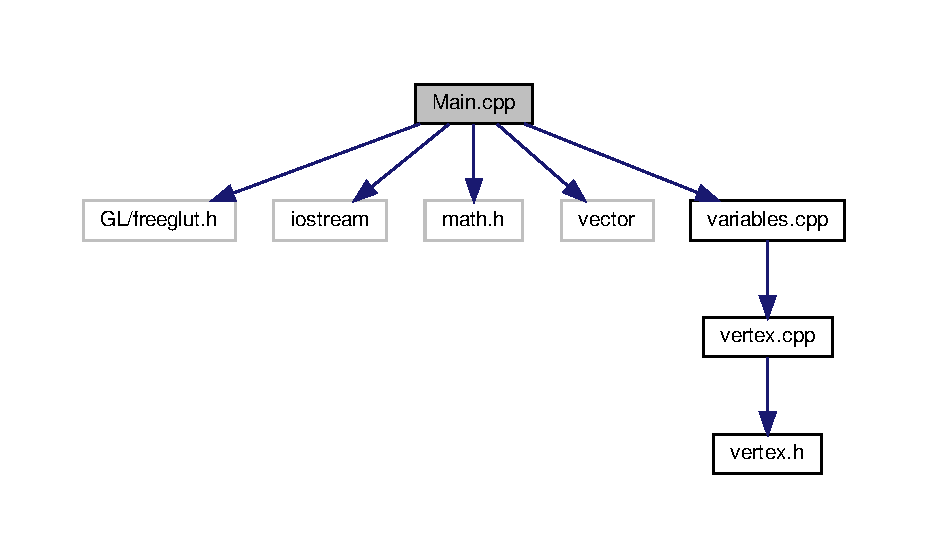
\includegraphics[width=350pt]{_main_8cpp__incl}
\end{center}
\end{figure}
\subsection*{Functions}
\begin{DoxyCompactItemize}
\item 
void \hyperlink{_main_8cpp_a1e5b20fed15743656bb6d2e6a6ea6269}{display} ()
\item 
void \hyperlink{_main_8cpp_a02fd73d861ef2e4aabb38c0c9ff82947}{init} ()
\item 
int \hyperlink{_main_8cpp_a3c04138a5bfe5d72780bb7e82a18e627}{main} (int argc, char $\ast$$\ast$argv)
\end{DoxyCompactItemize}


\subsection{Function Documentation}
\mbox{\Hypertarget{_main_8cpp_a1e5b20fed15743656bb6d2e6a6ea6269}\label{_main_8cpp_a1e5b20fed15743656bb6d2e6a6ea6269}} 
\index{Main.\+cpp@{Main.\+cpp}!display@{display}}
\index{display@{display}!Main.\+cpp@{Main.\+cpp}}
\subsubsection{\texorpdfstring{display()}{display()}}
{\footnotesize\ttfamily void display (\begin{DoxyParamCaption}{ }\end{DoxyParamCaption})}

Setting the colour aqua

Drawing all the points that are in our vector array of type vertex

Drawing the curve

White text \mbox{\Hypertarget{_main_8cpp_a02fd73d861ef2e4aabb38c0c9ff82947}\label{_main_8cpp_a02fd73d861ef2e4aabb38c0c9ff82947}} 
\index{Main.\+cpp@{Main.\+cpp}!init@{init}}
\index{init@{init}!Main.\+cpp@{Main.\+cpp}}
\subsubsection{\texorpdfstring{init()}{init()}}
{\footnotesize\ttfamily void init (\begin{DoxyParamCaption}{ }\end{DoxyParamCaption})}

Initializes GL states Called by main after window creation \mbox{\Hypertarget{_main_8cpp_a3c04138a5bfe5d72780bb7e82a18e627}\label{_main_8cpp_a3c04138a5bfe5d72780bb7e82a18e627}} 
\index{Main.\+cpp@{Main.\+cpp}!main@{main}}
\index{main@{main}!Main.\+cpp@{Main.\+cpp}}
\subsubsection{\texorpdfstring{main()}{main()}}
{\footnotesize\ttfamily int main (\begin{DoxyParamCaption}\item[{int}]{argc,  }\item[{char $\ast$$\ast$}]{argv }\end{DoxyParamCaption})}

Initialize Open\+G\+L/\+G\+L\+UT

Make a window

Initialize GL states \& register callbacks

The glut display function to render our scene to the window we made

Glut idle function is defines what happens when our screen is idle,i.\+e, we arent interacting with it

to implement our keyboard strokes and allow our keyboard to interact with the window

to maintain the aspect ratio on changing the size of our window

to allow our mouse interacting with the window 
\hypertarget{mouse_8cpp}{}\section{mouse.\+cpp File Reference}
\label{mouse_8cpp}\index{mouse.\+cpp@{mouse.\+cpp}}
\subsection*{Functions}
\begin{DoxyCompactItemize}
\item 
void \hyperlink{mouse_8cpp_ac76a5d78172a826cd6ee9512b89a86c0}{mouse} (int button, int state, int x, int y)
\end{DoxyCompactItemize}
\subsection*{Variables}
\begin{DoxyCompactItemize}
\item 
int \hyperlink{mouse_8cpp_a210b67113d562ea9ff67c719f2f441a5}{near\+Vtx}
\end{DoxyCompactItemize}


\subsection{Function Documentation}
\mbox{\Hypertarget{mouse_8cpp_ac76a5d78172a826cd6ee9512b89a86c0}\label{mouse_8cpp_ac76a5d78172a826cd6ee9512b89a86c0}} 
\index{mouse.\+cpp@{mouse.\+cpp}!mouse@{mouse}}
\index{mouse@{mouse}!mouse.\+cpp@{mouse.\+cpp}}
\subsubsection{\texorpdfstring{mouse()}{mouse()}}
{\footnotesize\ttfamily void mouse (\begin{DoxyParamCaption}\item[{int}]{button,  }\item[{int}]{state,  }\item[{int}]{x,  }\item[{int}]{y }\end{DoxyParamCaption})}

mouse The G\+L\+UT mouse function When left button of our mouse is pressed , we want to add a new point and change our bezier curve accordingly

Getting the x-\/y position of the cursor when the left button is clicked

We print out the co-\/ordinates to see that the axes and glut\+Ortho function is working correctly

Adding this to our original array of all the points as any point where the left click is pressed should be drawn and the bezier curve should be changed accordingly

When our right button of the mouse is pressed , we want to delete that point from our set of points to draw the bezier curve and hence the curve should be changed accordingly

Getting the x-\/y position of the cursor when the right button is clicked

We find the nearest point which is used to draw our bezier curve and remove that point. This is done because we cant always have pin point precision in removing a point.

Removing the point from our original vertex containing the points used to draw the bezier curve. After removing , we must update our bezier curve

Now we want to drag a point from the point where we click our middle button of our mouse and then draw it at the point where we release the middle button of our mouse

Getting the x-\/y position of the cursor when the middle button is clicked

We find the nearest point which is used to draw our bezier curve and select that point. This is done because we cant always have pin point precision in selecting a point.

Getting the x-\/y position of the cursor when the middle button is released

Now we change the point where our middle button was released in the original vertex vector and update the bezier curve accordingly

Save the mouse position 

\subsection{Variable Documentation}
\mbox{\Hypertarget{mouse_8cpp_a210b67113d562ea9ff67c719f2f441a5}\label{mouse_8cpp_a210b67113d562ea9ff67c719f2f441a5}} 
\index{mouse.\+cpp@{mouse.\+cpp}!near\+Vtx@{near\+Vtx}}
\index{near\+Vtx@{near\+Vtx}!mouse.\+cpp@{mouse.\+cpp}}
\subsubsection{\texorpdfstring{near\+Vtx}{nearVtx}}
{\footnotesize\ttfamily int near\+Vtx}


\hypertarget{_r_e_a_d_m_e_8md}{}\section{R\+E\+A\+D\+M\+E.\+md File Reference}
\label{_r_e_a_d_m_e_8md}\index{R\+E\+A\+D\+M\+E.\+md@{R\+E\+A\+D\+M\+E.\+md}}

\hypertarget{reshape_8cpp}{}\section{reshape.\+cpp File Reference}
\label{reshape_8cpp}\index{reshape.\+cpp@{reshape.\+cpp}}
\subsection*{Functions}
\begin{DoxyCompactItemize}
\item 
void \hyperlink{reshape_8cpp_acc1ffe65e6869931318610cae7210078}{reshape} (int w, int h)
\end{DoxyCompactItemize}


\subsection{Function Documentation}
\mbox{\Hypertarget{reshape_8cpp_acc1ffe65e6869931318610cae7210078}\label{reshape_8cpp_acc1ffe65e6869931318610cae7210078}} 
\index{reshape.\+cpp@{reshape.\+cpp}!reshape@{reshape}}
\index{reshape@{reshape}!reshape.\+cpp@{reshape.\+cpp}}
\subsubsection{\texorpdfstring{reshape()}{reshape()}}
{\footnotesize\ttfamily void reshape (\begin{DoxyParamCaption}\item[{int}]{w,  }\item[{int}]{h }\end{DoxyParamCaption})}

reshape function. This is to ensure that the aspect ratio is maintained even when we change the window size Set the viewport to be the entire drawing area of the window

Save the window size

Set up the projection

Always go back to model/view mode 
\hypertarget{variables_8cpp}{}\section{variables.\+cpp File Reference}
\label{variables_8cpp}\index{variables.\+cpp@{variables.\+cpp}}
{\ttfamily \#include \char`\"{}vertex.\+cpp\char`\"{}}\newline
Include dependency graph for variables.\+cpp\+:\nopagebreak
\begin{figure}[H]
\begin{center}
\leavevmode
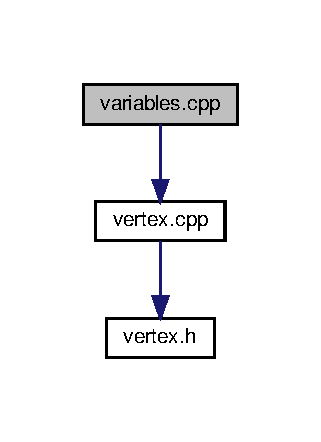
\includegraphics[width=154pt]{variables_8cpp__incl}
\end{center}
\end{figure}
This graph shows which files directly or indirectly include this file\+:\nopagebreak
\begin{figure}[H]
\begin{center}
\leavevmode
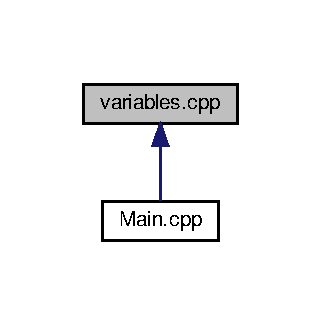
\includegraphics[width=154pt]{variables_8cpp__dep__incl}
\end{center}
\end{figure}
\subsection*{Variables}
\begin{DoxyCompactItemize}
\item 
\hyperlink{classvertex}{vertex} \hyperlink{variables_8cpp_a8e51567ce3a58dfdf38ffe21f9a504ab}{obj}
\item 
const int \hyperlink{variables_8cpp_acb393dd3d895d00164d74496ebe19db4}{startwinsize} = 600
\item 
int \hyperlink{variables_8cpp_a6e0c3613356826aa5d156663a089bf34}{winw}
\item 
int \hyperlink{variables_8cpp_aab52af402fcd036d4520b205699fb08d}{winh}
\item 
bool \hyperlink{variables_8cpp_aa130fef5d9ce85c4ec54864d54f466da}{mouseleftdown} = false
\item 
int \hyperlink{variables_8cpp_aa3d2105adcc19a5aba525c805fc49ff2}{mousex}
\item 
int \hyperlink{variables_8cpp_a6d4a0453f23b7c4df1a7be2972529a0b}{mousey}
\item 
const int \hyperlink{variables_8cpp_a612d5955814d9f21250771c13abeaa7d}{E\+S\+C\+K\+EY} = 27
\item 
const double \hyperlink{variables_8cpp_ac0f8a103d0b0f3d64599b1b5fb40a880}{pointsize} = 40
\end{DoxyCompactItemize}


\subsection{Variable Documentation}
\mbox{\Hypertarget{variables_8cpp_a612d5955814d9f21250771c13abeaa7d}\label{variables_8cpp_a612d5955814d9f21250771c13abeaa7d}} 
\index{variables.\+cpp@{variables.\+cpp}!E\+S\+C\+K\+EY@{E\+S\+C\+K\+EY}}
\index{E\+S\+C\+K\+EY@{E\+S\+C\+K\+EY}!variables.\+cpp@{variables.\+cpp}}
\subsubsection{\texorpdfstring{E\+S\+C\+K\+EY}{ESCKEY}}
{\footnotesize\ttfamily const int E\+S\+C\+K\+EY = 27}

Mouse x,y coords, in G\+L\+UT format (pixels from upper-\/left corner). Only guaranteed to be valid if a mouse button is down. Saved by mouse, motion. Keyboard \mbox{\Hypertarget{variables_8cpp_aa130fef5d9ce85c4ec54864d54f466da}\label{variables_8cpp_aa130fef5d9ce85c4ec54864d54f466da}} 
\index{variables.\+cpp@{variables.\+cpp}!mouseleftdown@{mouseleftdown}}
\index{mouseleftdown@{mouseleftdown}!variables.\+cpp@{variables.\+cpp}}
\subsubsection{\texorpdfstring{mouseleftdown}{mouseleftdown}}
{\footnotesize\ttfamily bool mouseleftdown = false}

Window width \& height, in pixels, saved by reshape Mouse \mbox{\Hypertarget{variables_8cpp_aa3d2105adcc19a5aba525c805fc49ff2}\label{variables_8cpp_aa3d2105adcc19a5aba525c805fc49ff2}} 
\index{variables.\+cpp@{variables.\+cpp}!mousex@{mousex}}
\index{mousex@{mousex}!variables.\+cpp@{variables.\+cpp}}
\subsubsection{\texorpdfstring{mousex}{mousex}}
{\footnotesize\ttfamily int mousex}

True if mouse L\+E\+FT button is down./$\ast$$\ast$glut\+Motion\+Func(motion); Do something Saved by mouse. \mbox{\Hypertarget{variables_8cpp_a6d4a0453f23b7c4df1a7be2972529a0b}\label{variables_8cpp_a6d4a0453f23b7c4df1a7be2972529a0b}} 
\index{variables.\+cpp@{variables.\+cpp}!mousey@{mousey}}
\index{mousey@{mousey}!variables.\+cpp@{variables.\+cpp}}
\subsubsection{\texorpdfstring{mousey}{mousey}}
{\footnotesize\ttfamily int mousey}

\mbox{\Hypertarget{variables_8cpp_a8e51567ce3a58dfdf38ffe21f9a504ab}\label{variables_8cpp_a8e51567ce3a58dfdf38ffe21f9a504ab}} 
\index{variables.\+cpp@{variables.\+cpp}!obj@{obj}}
\index{obj@{obj}!variables.\+cpp@{variables.\+cpp}}
\subsubsection{\texorpdfstring{obj}{obj}}
{\footnotesize\ttfamily \hyperlink{classvertex}{vertex} obj}

\mbox{\Hypertarget{variables_8cpp_ac0f8a103d0b0f3d64599b1b5fb40a880}\label{variables_8cpp_ac0f8a103d0b0f3d64599b1b5fb40a880}} 
\index{variables.\+cpp@{variables.\+cpp}!pointsize@{pointsize}}
\index{pointsize@{pointsize}!variables.\+cpp@{variables.\+cpp}}
\subsubsection{\texorpdfstring{pointsize}{pointsize}}
{\footnotesize\ttfamily const double pointsize = 40}

A\+S\+C\+II value of escape character Other \mbox{\Hypertarget{variables_8cpp_acb393dd3d895d00164d74496ebe19db4}\label{variables_8cpp_acb393dd3d895d00164d74496ebe19db4}} 
\index{variables.\+cpp@{variables.\+cpp}!startwinsize@{startwinsize}}
\index{startwinsize@{startwinsize}!variables.\+cpp@{variables.\+cpp}}
\subsubsection{\texorpdfstring{startwinsize}{startwinsize}}
{\footnotesize\ttfamily const int startwinsize = 600}

Global variables Window/viewport \mbox{\Hypertarget{variables_8cpp_aab52af402fcd036d4520b205699fb08d}\label{variables_8cpp_aab52af402fcd036d4520b205699fb08d}} 
\index{variables.\+cpp@{variables.\+cpp}!winh@{winh}}
\index{winh@{winh}!variables.\+cpp@{variables.\+cpp}}
\subsubsection{\texorpdfstring{winh}{winh}}
{\footnotesize\ttfamily int winh}

\mbox{\Hypertarget{variables_8cpp_a6e0c3613356826aa5d156663a089bf34}\label{variables_8cpp_a6e0c3613356826aa5d156663a089bf34}} 
\index{variables.\+cpp@{variables.\+cpp}!winw@{winw}}
\index{winw@{winw}!variables.\+cpp@{variables.\+cpp}}
\subsubsection{\texorpdfstring{winw}{winw}}
{\footnotesize\ttfamily int winw}

Starting window width \& height, in pixels 
\hypertarget{vertex_8cpp}{}\section{vertex.\+cpp File Reference}
\label{vertex_8cpp}\index{vertex.\+cpp@{vertex.\+cpp}}
{\ttfamily \#include \char`\"{}vertex.\+h\char`\"{}}\newline
Include dependency graph for vertex.\+cpp\+:\nopagebreak
\begin{figure}[H]
\begin{center}
\leavevmode
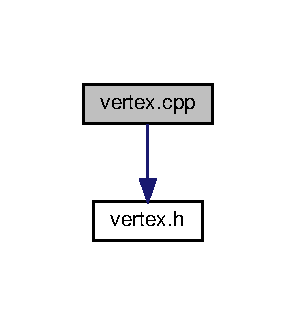
\includegraphics[width=142pt]{vertex_8cpp__incl}
\end{center}
\end{figure}
This graph shows which files directly or indirectly include this file\+:\nopagebreak
\begin{figure}[H]
\begin{center}
\leavevmode
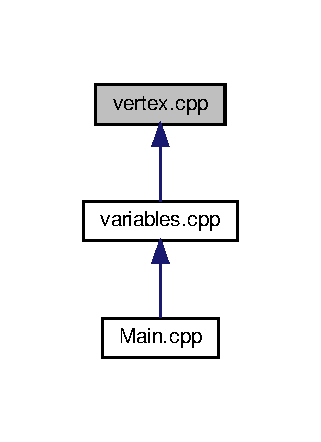
\includegraphics[width=154pt]{vertex_8cpp__dep__incl}
\end{center}
\end{figure}

\hypertarget{vertex_8h}{}\section{vertex.\+h File Reference}
\label{vertex_8h}\index{vertex.\+h@{vertex.\+h}}
This graph shows which files directly or indirectly include this file\+:\nopagebreak
\begin{figure}[H]
\begin{center}
\leavevmode
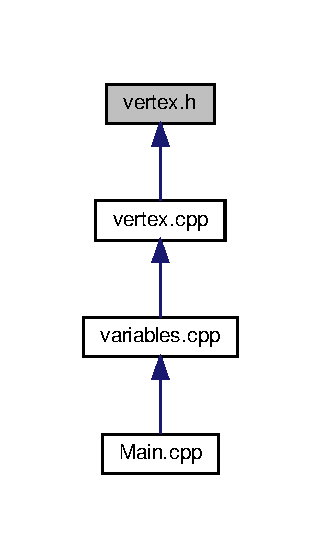
\includegraphics[width=154pt]{vertex_8h__dep__incl}
\end{center}
\end{figure}
\subsection*{Classes}
\begin{DoxyCompactItemize}
\item 
class \hyperlink{classvertex}{vertex}
\end{DoxyCompactItemize}

%--- End generated contents ---

% Index
\backmatter
\newpage
\phantomsection
\clearemptydoublepage
\addcontentsline{toc}{chapter}{Index}
\printindex

\end{document}
